\subsection*{Operating System Interaction with NVMe SSD}
The operating system communicates with an NVMe SSD through a layered I/O architecture. When an application issues a read or write request, it passes through the Virtual File System (VFS), block I/O layer, and I/O scheduler before reaching the NVMe driver. The driver converts the request into NVMe commands, places them in submission queues, and transfers them to the SSD controller over the PCIe interface using Direct Memory Access (DMA). The controller processes the commands, accesses the NAND flash memory through the Flash Translation Layer (FTL), and performs functions such as wear leveling, garbage collection, and error correction. After the operation is completed, the controller updates the completion queue and notifies the operating system through an interrupt. This queue-based architecture enables efficient parallel processing of I/O requests, resulting in lower latency and higher throughput than traditional SATA-based storage devices.

\begin{figure}[H]
    \centering
     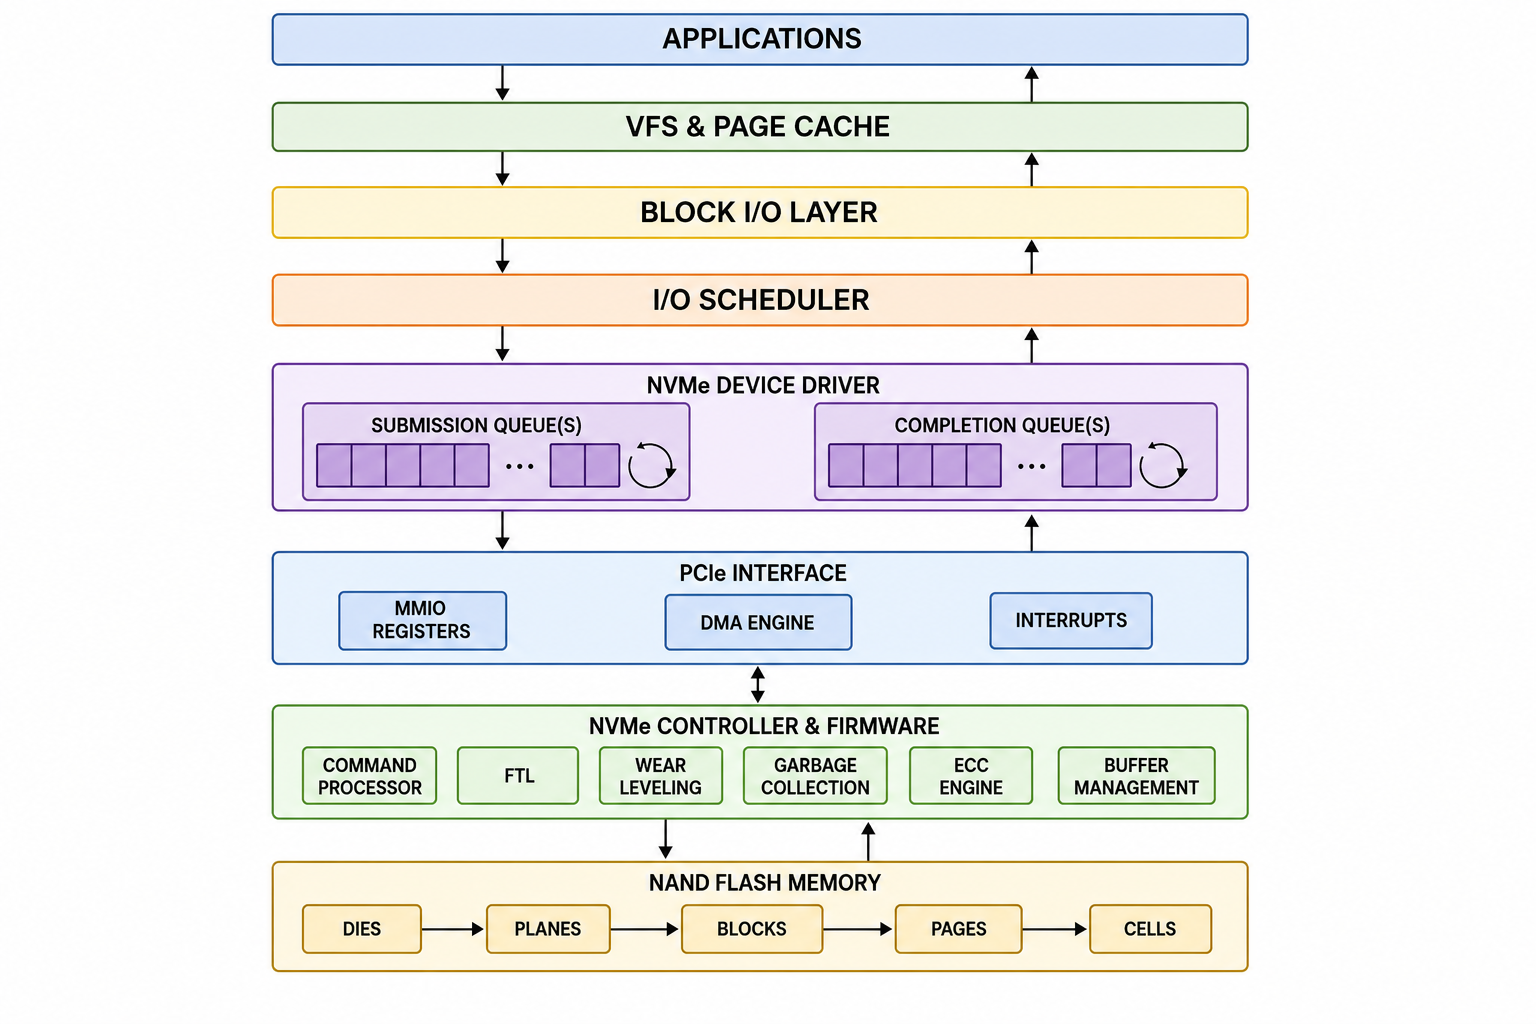
\includegraphics[width=1\textwidth]{os interaction with nvme.png}
    \caption{OS interaction with NVMe}
    \cite{_nvme_architecture}
    \label{fig: nvme and os } 
\end{figure}
\newpage